
\section{Intersection Theory}\label{sec:intersection-theory}

Throughout this chapter, we'll adopt the convention that $X$ is an ambient $n$-dimensional oriented manifold with boundary, and $M$ and $N$ are closed manifolds. We'll assume that all closed submanifolds of $X$ and smooth maps from a closed manifold to $X$ avoid the boundary.

\begin{definition}\label{def:transverse-intersection-basic}
	Two submanifolds $M,N\subset X$ are said to \defn{intersect tranversally} or to be \defn{transverse} if for all points $p\in M\cap N$ we have $\T_p M\oplus \T_p N = \T_p X$.
\end{definition}

\begin{figure}[ht]
	\centering
	\import{graphics/temp-diagrams/}{transverse-intersection.pdf_tex}
	\medskip
	\caption{Examples and non-examples of transverse intersections in $\R^3$.}\label{fig:transverse-intersection}
\end{figure}

If we lose the assumption that the spaces we're considering aren't smoothly embedded submanifolds of the ambient space, but rather images of a smooth map then this definition can be slightly generalized.

\begin{definition}\label{def:transverse-intersection}
	If $f : N \to X$ and $g : M \to X$ are smooth maps, we say that $f$ and $g$ are \defn{transverse} if for all $p\in N$ and $q\in M$ with $f(p)=g(q)=x\in X$, we have
	\[
		\T_x X = df_p(\T_p N) \oplus dg_q(\T_q M).
	\]
\end{definition}

\begin{remark}
	When $f$ and $g$ are embeddings, this recovers \cref{def:transverse-intersection-basic}.
\end{remark}

While it's easy to come up with examples of manifolds which aren't transverse, there is a mathematical sense in which ``almost all'' submanifolds intersect transversally.

\begin{theorem}
	Let $C^\infty(N,X)$ be the space of all maps from a compact manifold $N$ to some ambient manifold $X$. If we fix a submanifold $M\subset X$, then the subset
	\[
		C^\infty_{\mathrm{tv.}\,M}(N,X)=\{ f : N \to X \mid f\textrm{ is transverse to } M\}\subset C^\infty(N,X)
	\]
	of maps transverse to $M$ is a dense subset of $C^\infty(N,X)$.
\end{theorem}

\begin{proof}
	See the proof of Theorems~6.35 in \cite{lee2012smooth}.
\end{proof}

In simpler terms, this density of transverse maps implies that transversality is a \defn{stable}[stable property] and \defn{generic}[generic property] property. Stability in this context means that it is resilient to perturbations (if a map is transverse to $M$, perturbing it slightly will keep it transverse to $M$), and generality means that if a map is not transverse to $M$, we can perturb it slightly to make it transverse.
What this means for us is that without much loss of generality, we can assume that all manifolds and smooth maps intersect transversally.

\begin{figure}[ht]
	\centering
	\import{graphics/temp-diagrams/}{perturbing-intersection-transverse.pdf_tex}
	\medskip
	\caption{Perturbing a manifold embedding to get a transverse intersection.}\label{fig:perturbing-intersections-transverse}
\end{figure}

The observant reader might remark that there isn't a way of measuring distances between maps in $C^\infty(N,X)$, this would require more than just the topological data we have access to. We do however have a notion of homotopy, so whenever refer to stability, generality, and perturbation, we use the following formal definition.

\begin{definition}
	Suppose we have a property $\mathcal{P}$ of functions between topological spaces.
	\begin{enumerate}
		\item The property $\mathcal{P}$ is said to be \defn{stable}[stable property] if for every function $f : X \to Y$ satisfying $\mathcal{P}$ and homotopy $H : X\times[0,1]\to Y$ with $H(x,0) = f(x)$, there exists an $\varepsilon>0$ such that for all $s\in [0,\varepsilon)$, the function $H(x,s)$ also satisfies $\mathcal{P}$.
		\item The property $\mathcal{P}$ is said to be \defn{generic}[generic property] if for every function $f : X \to Y$ \emph{not} satisfying $\mathcal{P}$ and arbitrary $\varepsilon>0$, there is a homotopy $H : X\times [0,\varepsilon] \to Y$ with $H(x,0)=f(x)$ such that the function $H(x,\varepsilon)$ satisfies $\mathcal{P}$.
	\end{enumerate}
\end{definition}

\subsection{The Oriented Intersection Number}

One of the fundamental properties concerning transverse maps is that they behave well when taking intersections, or more generally when taking preimages. This forms the backbone of the intersection theory of manifolds.

\begin{theorem}[Preimage Theorem]\label{thm:preimage}
	If $f : N \to X$ is a smooth map transverse to a submanifold $M\subset X$ then $S=f^{-1}(M)\subset N$ is a submanifold with the same codimension in $N$ as $M$ in $X$.
\end{theorem}
\begin{proof}
	See the proof of Theorem~6.30 in \cite{lee2012smooth}.
\end{proof}

\begin{remark}\label{rmk:symmetric-preimage-theorem}
	We can get a symmetric version of this theorem as a straightforward corollary. If we have two transverse maps $f : N\to X$ and $g : M\to X$, then the map $f\times g : N\times M \to X\times X$ is transverse to the diagonal submanifold $\Delta\subset X\times X$. \cref{thm:preimage} will then imply that
	\[
		(f\times g)^{-1}(\Delta) \subset M\times N
	\]
	is a submanifold. When $g$ is an embedding, $(f\times g)^{-1}(\Delta)$ can be projected down onto $M$ to get the preimage $f^{-1}(M)$.
\end{remark}

If the manifolds involved in \cref{thm:preimage} are orientable, this preimage $S$ admits a canonical orientation by the following procedure. First of all, recall that for any embedded manifold $M\subset X$ there is an exact sequence of vector bundles by quotienting
\begin{equation}\label{eq:oriented-intersection-number-1}
	\begin{tikzcd}
		0 & {\T M} & {\T X} & {\T X/M} & 0
		\arrow[from=1-1, to=1-2]
		\arrow[from=1-2, to=1-3]
		\arrow[from=1-3, to=1-4]
		\arrow[from=1-4, to=1-5]
	\end{tikzcd}
\end{equation}
where $\T X/M$ is the normal bundle of $M\subset X$. Using the orientations of $X$ and $M$, we can use this exact sequence to get an orientation of the normal bundle $\T X/M$. At every point $p\in S$ of the preimage, the differential map $df$ connects the sequence \cref{eq:oriented-intersection-number-1} to the normal bundle sequence for the embedding $S\subset N$.
\begin{equation}\label{eq:oriented-intersection-number-2}
	\begin{tikzcd}
		0 & {\T_pS} & {\T_p N} & {\T_p N/S} & 0 \\
		0 & {\T_{f(p)}M} & {\T_{f(p)}X} & {\T_{f(p)}X/M} & 0
		\arrow[from=1-1, to=1-2]
		\arrow[from=1-2, to=1-3]
		\arrow["{df_p}", from=1-2, to=2-2]
		\arrow[from=1-3, to=1-4]
		\arrow["{df_p}", from=1-3, to=2-3]
		\arrow[from=1-4, to=1-5]
		\arrow["{df_p}", from=1-4, to=2-4]
		\arrow[from=2-1, to=2-2]
		\arrow[from=2-2, to=2-3]
		\arrow[from=2-3, to=2-4]
		\arrow[from=2-4, to=2-5]
	\end{tikzcd}
\end{equation}
In this diagram \cref{eq:oriented-intersection-number-2}, the rightmost vertical map is an isomorphism by the transversality of $f$ and $M$. This means that we can pullback the orientation on $\T_{f(p)} X/M$ to $\T_p N/S$. Since $\T_p N$ is oriented, the usual ``2-out-of-3'' rule applied to the top row of \cref{eq:oriented-intersection-number-2} gives an orientation of $\T_p S$. See \cref{fig:preimage-orientation} for an example of this orienting procedure.

\begin{figure}[ht]
	\centering
	\import{graphics/temp-diagrams/}{preimage-orientation.pdf_tex}
	\medskip
	\caption{Orienting a preimage (assuming a clockwise orientation on $X$ and $N$).}\label{fig:preimage-orientation}
\end{figure}

When $M$ and $N$ have complementary dimensions, the preimage $S=f^{-1}(N)\subset M$ is a compact oriented $0$-dimensional manifold. For each point $p\in S$, we have $\T_p S=0$ so the map $\T_p N\to \T_p N/S$ in \cref{eq:oriented-intersection-number-2} is an isomorphism. The orientation of $N$ gives an orientation of $\T_p N$, and the preimage orientation procedure gives us an orientation of $\T_p N/S$. Now we can define:

\begin{definition}
	The \defn{local (oriented) intersection number}[oriented intersection number (local)] of $f$ and $M$ at $p\in S$ is
	\[
		\#_p^X(f, M) = \begin{cases}
			+1 & \T_p N/S \textrm{ has the same orientation as } \T_p N,     \\
			-1 & \T_p N/S \textrm{ has the opposite orientation to } \T_p N.
		\end{cases}
	\]
\end{definition}
Summing over all of the local intersection numbers gives a global quantity.
\begin{definition}
	The \defn{(oriented) intersection number}[oriented intersection number] of a smooth map $f : N \to X$ intersecting a submanifold $M\subset X$ transversally is
	\[
		\#^X(f, M) = \sum_{p\in S} \#_p^X(f, M) \in \Z.
	\]
\end{definition}

\begin{remark}\label{rmk:symmetric-intersection-number}
	For a more symmetric version of this definition when two smooth maps $f : N \to X$ and $g : M \to X$ intersect transversally, we could take inspiration from \cref{rmk:symmetric-preimage-theorem} and define the oriented intersection number of the smooth maps $f$ and $g$ as
	\[
		\#^X(f,g) = \#^{X\times X}(f\times g, \Delta).
	\]
	This symmetric intersection number is graded commutative in the dimensions of $M$ and $N$, i.e.
	\begin{equation}\label{eq:intersection-number-graded-commutative}
		\#^X(f,g) = (-1)^{\dim M\cdot \dim N} \#^X(g,f)
	\end{equation}
\end{remark}

Just as the property of transversality is stable -- resilient to homotopic perturbations -- so too is the oriented intersection number. This follows as a corollary to a more general theorem.

\begin{theorem}
	If $W$ is a compact oriented manifold with boundary, and $H : W \to X$ is a smooth map, then $\#^X(\partial H, M)=0$. Here, we use the notation $\partial H : \partial W \to X$ to refer to the restriction of $H$ to the boundary of $W$.
\end{theorem}

\begin{corollary}
	If $H : [0,1]\times N \to X$ is a smooth homotopy, then $\#^X(H_0, M) = \#^X(H_1, M)$.
\end{corollary}

Applying the construction of the symmetric oriented intersection number gives a map
\begin{equation}\label{eq:oriented-intersection-number-homotopy}
	\lkxfunc{\#^X}{[N,X]\times [M,X]}{\Z}{f,g}{\#^X(f,g)}
\end{equation}
This is a geometric precursor to the intersection form of a manifold, a central object of study in geometric topology.

\begin{remark}
	If we don't assume orientations, we can still get a homotopy invariant intersection number, however we must reduce mod $2$. In this case, we could simply define 
	\[
		\#_2^X(f,M) = |S|\mod 2.
	\]
	This is called the \defn{unoriented intersection number}.
	\todo{elaborate}
\end{remark}

Finally, we'll state a useful result in computer self-intersection numbers -- a way to compute the intersection number of a submanifold with itself.

\begin{theorem}\label{thm:euler-number-self-intersection}
	If $M$ is a closed $m$-dimensional submanifold of a $2m$-dimensional submanifold $X$ then we have
	\[
		\#^X(M, M) = \chi(\T X/M)
	\]
	where $\chi(\T X/M)$ is the Euler number of the normal bundle of $M$.
\end{theorem}
\begin{proof}
	\todo{todo}
\end{proof}

\begin{corollary}\label{thm:euler-number-self-intersection-corollary}
	The Euler number $\chi(\xi)$ of an oriented real vector bundle $\xi : E \to B$ over a compact oriented manifold can be expressed as the intersection number
	\[
		\#^E(z,z) = \chi(\xi)
	\]
	where $z : B \to E$ is the zero section.
\end{corollary}

\todo{add 1.C from \cite{levine1985lectures}}

\subsection{Homology Classes and Submanifolds}

Let $f : N\subset X$ be a smooth map from a compact oriented $p$-dimensional manifold $N$ to $X$. The data of an orientation on a closed manifold gives a fundamental class $[N]\in \H_p(N)$ which can be pushed forward along the map $f : N \hookrightarrow X$ to give us a homology class $f_* [N]\in \H_p(X)$. This is the homology class associated to a smooth map $N\to X$.
This correspondence behaves nicely with respect to perturbations, and thus as we will later see, with transversality.
Suppose $H : N\times [0,1] \to X$ is a homotopy with $H(x,0)=f(x)$ which perturbs the map $f$. For any $\varepsilon>0$, the map $f_\varepsilon : N \to X$ given by $f_\varepsilon(x)=H(x,\varepsilon)$ is homotopic to $f$ and hence induces the same map on homology $\H_p(N)\to \H_p(X)$. The homology class associated to a map $f : N \to X$ thus solely depends on the homotopy type of $f$ so we get a map
\[
	\lkxfunc{}{[N,X]}{\H_p(X).}
\]
Letting $N=S^p$, we can see that this is a generalization of the Hurewicz homomorphism which links homotopy groups to homology groups via a map $\pi_p(X) \to \H_p(X)$.
As with the Hurewicz homomorphism, this correspondence is generally not surjective or injective. If a space is $k$-connected for $k\geq 1$ then we have a Hurewicz isomorphism $\pi_{k+1}(X) \to \H_{k+1}(X)$ which means that every homology cycle in $\H_{k+1}(X)$ can at least be represented by a smooth map of a sphere $S^{k+1}$ into $X$. This smooth map might have ``double-points'', i.e. when multiple points of the sphere map to the same point in the image and prevent the smooth map from being an embedding.

\begin{example}
	In the punctured plane $X=\R^2\setminus \{0\}$ with homology $\H_1(X)\cong \Z$, the only homology cycles which can be represented by embedded submanifolds are $0,\pm 1$, by a circle not containing the origin and circles of both orientations surrounding the origin respectively. A smooth map representing a cycle of higher degree would necessarily have a double-point as in \cref{fig:double-point}.
\end{example}

\begin{figure}[ht]
	\centering
	\import{graphics/temp-diagrams/}{double-point.pdf_tex}
	\caption{A double-point in a smooth map representing $\pm 2\in \H_1(\R^2\setminus\{0\})$.}\label{fig:double-point}
\end{figure}

That being said, many specially constructed manifolds we will consider in this chapter will at least have a basis by embedded submanifolds, and every homology class will admit a representation by a smooth map. For a classical account of some issues that can arise when representing homology classes by smooth maps, see Chapter II of Ren\'e Thom's seminal paper \cite{thom1954}.

\begin{remark}
	In some special cases, homology classes can \emph{always} be represented by embedded submanifolds. For instance, if $X$ is a $4$-manifold, there are isomorphisms
	\[
		\H^2(X; \Z) \cong [X, K(\Z,2)] \cong [X, \CP^\infty] \cong [X,\CP^2],
	\]
	where the first is the representability of singular cohomology by the Eilenberg-Maclane spectrum, the second identifies $\CP^\infty$ as a $K(\Z,2)$ space, and the third uses the cellular approximation theorem. Any cohomology cycle $\omega\in \H^2(X)$ can be represented by a smooth function $f : X \to \CP^2$. If we choose this function to be transverse to $\CP^1\subset \CP^2$, then $f^{-1}(\CP^1)$ is an embedded $2$-dimensional submanifold of $X$ which corresponds to a Poincar\'e dual class to $\omega$. When $X$ is a compact manifold, Poincar\'e duality tells us that all $2$-dimensional homology cycles can be represented by embedded submanifolds in this way. This is one reason why $4$-manifolds (especially simply-connected $4$-manifolds) are such wonderful geometric objects of study!
\end{remark}

\subsection{Homology Intersection}

Now let's see if our previously defined notion of an oriented intersection number transfers over as an operation on homology classes. Recall that by the Poincar\'e-Lefschetz duality for compact manifolds with boundary, there is an isomorphism
\[
	\lkxfunc{}{\H^{n-p}(X,\partial X)}{\H_p(X)}{\omega}{\omega\frown [X,\partial X]}
\]
given an orientation class $[X,\partial X]\in \H_n(X, \partial X)$. Under this duality, there is a geometric interpretation of the cup product on cohomology cycles as the oriented intersection number for submanifolds representing the dual homology cycles (when such a representation is possible). We can define this homology intersection pairing $\tnsv$ as the top map in the commutative square
\begin{equation}\label{eq:homology-intersection}
	\begin{tikzcd}
		{\H_p(X)\otimes \H_q(X)} & {\H_{n-p-q}(X)} \\
		{\H^{n-p}(X, \partial X)\otimes \H^{n-q}(X,\partial X)} & {\H^{2n-p-q}(X,\partial X)}
		\arrow["\tnsv", from=1-1, to=1-2]
		\arrow[tail reversed, from=1-1, to=2-1]
		\arrow[tail reversed, from=1-2, to=2-2]
		\arrow["\smile", from=2-1, to=2-2]
	\end{tikzcd}
\end{equation}
where the vertical maps are the Poincar\'e-Lefschetz isomorphism. Finally, we have our link between the algebra of (co)homology and the differential topology of intersections.

\begin{theorem}
	Suppose $M,N\subset X$ are transverse oriented submanifolds. Then we have
	\[\iota_*[M]\tnsv \iota_*[N] = \#_X(M,N)\]
\end{theorem}
\begin{proof}
	\todo{todo}
\end{proof}

As suggested by the map in \cref{eq:oriented-intersection-number-homotopy}, we now have an entirely algebraic object which encapsulates the geometry of intersections on a manifold.

\todo{link, this used to be part of chapter 2}

Since $\smile$ is graded-commutative, by \cref{eq:homology-intersection} so is $\tnsv$. Of course, we would expect the graded-commutativity as a generalization of \cref{eq:intersection-number-graded-commutative}. This implies:

\section{Vector Bundles Over Spheres}\label{sec:vector-bundles-over-spheres}

This is a good time for a brief interlude on vector bundles over spheres.
Vector bundles over a sphere can be classified by the clutching construction. Suppose $\xi : E \to S^m$ is a vector bundle. We can decompose the sphere $S^m$ into hemispheres $S^m=D_+^m\cup D_-^m$, and these disks intersect at the equator $D_+^m\cap D_-^m=S^{m-1}\subset S^m$ -- a sphere one dimension lower. The bundle $\xi$ can be trivialized on the hemispheres since they are contractible, and we denote these trivializations
\[
	\lkxfunc{\varphi_+}{E|_{D^m_+}}{D^m_+\times \R^m}
	\quad\textrm{and}\quad
	\lkxfunc{\varphi_-}{E|_{D^m_-}}{D_-^m \times \R^m.}\]
The trivializations must come with transition functions on their intersection (we might have to expand the intersection a bit so that it is open). The transition function is a diffeomorphism $\psi$ in the commutative diagram
\[\begin{tikzcd}
		{S^{m-1}\times \R^m} && {S^{m-1}\times \R^m} \\
		& {E|_{S^{m-1}}}
		\arrow["\psi", from=1-1, to=1-3]
		\arrow["{\varphi_+|_{S^{m-1}}}", from=2-2, to=1-1]
		\arrow["{\varphi_-|_{S^{m-1}}}"', from=2-2, to=1-3]
	\end{tikzcd}\]
which is constant on the first factor, and linear in the second factor. For each point $p\in S^{m-1}$, the diffeomorphism $\psi$ thus gives a linear function $\tau_p : \R^m \to \R^m$. These linear maps are the ``change of coordinate'' transformations between the fibers on the boundaries of $D_+^m$ and $D_-^m$ (see \cref{fig:clutching-construction}).
\begin{figure}[ht]
	\centering
	\import{graphics/temp-diagrams/}{clutching-construction.pdf_tex}
	\caption{Getting a map $\tau : S^{m-1}\to \GL_m$ from a vector bundle over $S^{m}$.}\label{fig:clutching-construction}
\end{figure}

Altogether, this family of linear transformations is indexed by the equator $S^{m-1}$, and this gives us a smooth map $\tau : S^{m-1}\to \GL_m$. It follows that the homotopy type of $\tau$ is only dependent on the isomorphism type of the bundle $\xi$ since any vector bundle isomorphism can be shown to induce a homotopy of smooth maps. In order words, we have a map
\[
	\lkxfunc{}{\op{Vect}_m(S^m)}{\pi_{m-1}(\GL_m).}
\]
sending a vector bundle $\xi$ to the its associated homotopy class $\tau\in \pi_{m-1}(\GL_m)$.

The construction works in the opposite direction as well. Whenever we have a homotopy class $\tau\in \pi_{m-1}(\GL_m)$, we can form a bundle $\xi_\tau : E_\tau \to S^{m}$ by letting
\[
	E_\tau = (D_+^m\times D^m)\cup_T (D_-^{m}\times D^m),
\]
where $T(x,y)=(x,\tau(x)y)$ is the glueing map.

\todo{write this}

A similar argument holds when we restrict to oriented bundles, i.e. vector bundles with structure group $\SO_m$.

\begin{theorem}
	The clutching construction gives bijections
	\[
		\begin{aligned}
			\lkxfunc{}{\pi_{m-1}(\O_m)}{\op{Vect}_m(S^m)} \\
			\lkxfunc{}{\pi_{m-1}(\SO_m)}{\op{Vect}_m^+(S^m)}
		\end{aligned}
	\]
	between homotopy groups of the orthogonal groups and isomorphism classes of vector bundles.
\end{theorem}
\begin{proof}
	\todo{prove}
\end{proof}

Under this correspondence the Euler number of a vector bundle can be considered as a group homomorphism
\[
	\lkxfunc{e}{\pi_{m-1}(\SO_m)}{\Z}{\tau}{e(\xi_\tau)}
\]
\begin{theorem}\label{thm:euler-number-of-vector-bundle-over-sphere}
	Let $p : \SO_{2m} \to \SO_{2m}/\SO_{2m-1}= S^{2m-1}$ be the projection map of the special orthogonal group to the sphere. Then the following diagram commutes,
	\[\begin{tikzcd}
			{\pi_{2m-1}(\SO_{2m})} & \Z \\
			{\pi_{2m-1}(S^{2m-1})}
			\arrow["e", from=1-1, to=1-2]
			\arrow["{p_*}"', from=1-1, to=2-1]
			\arrow[from=2-1, to=1-2]
		\end{tikzcd}\]
	where $\pi_{2m-1}(S^{2m-1})\to \Z$ is the degree isomorphism.
\end{theorem}
\begin{proof}
	\todo{prove}
\end{proof}

\begin{corollary}\label{cor:expressible-euler-numbers-spheres}
	The image of $e : \pi_{2m-1}(\SO_{2m})\to\Z$ is $2\Z$.
\end{corollary}
\begin{proof}
	\todo{prove}
\end{proof}

\begin{remark}
	The clutching construction is a special case of a more general classification of principal $G$-bundles. Generally, if $G$ is a Lie group there is a natural isomorphism of contravariant functors
	\[
		[-, \Bclass G] \lkxto \Bun_G(-)
	\]
	where $[-, \Bclass G]$ is the set of homotopy classes of maps to a space $\Bclass G$ and $\Bun_G(-)$ is the set of isomorphism classes of principal $G$-bundles over a given space.
	The space $\Bclass G$ is known as the \defn{classifying space}\footnote{The classifying space is rarely a manifold, and is usually an infinite dimensional CW complex.} of $G$ and this space comes equipped with a \defn{universal bundle} $\zeta : \Eclass G \to \Bclass G$. With this universal bundle, the natural isomorphism is easy to describe. Under the appropriate topological restrictions, a map $\tau : X \to \Bclass G$ gives us a pullback bundle $\tau^*\zeta$ over $X$. This is a principal $G$-bundle over $X$ which is entirely determined by the homotopy type of the \defn{classifying map} $\tau$.

	In some sense, the universal bundle $\zeta$ is the ``most twisted $G$-bundle''. Pullbacks of bundles generally ``dilute'' the twistedness of a bundle -- for instance, the splitting principle allows any complex vector bundle to be pulled back to a direct sum of complex line bundles. It would stand to reason that every bundle is the pullback of a more twisted bundle, and the limit of this process is the universal bundle $\zeta$ over the classifying space. See Chapter IV of \cite{botttu1982differential} for a wonderful exposition on the topic.

	It can be shown that (under suitable topological restrictions) there is a homotopy equivalence $\Omega \Bclass G \simeq G$ where $\Omega$ denotes the loop space operator in homotopy theory. Indeed from a homotopy theory perspective, the classifying space is a ``delooping'' of the group $G$. For spheres, the loop space suspension adjunction gives us natural isomorphisms
	\[
		\begin{aligned}
			\Bun_{G}(S^m) & \cong [S^m, \Bclass G]            \\
			              & \cong [\Sigma S^{m-1}, \Bclass G] \\
			              & \cong [S^{m-1}, \Omega\Bclass G]  \\
			              & \cong [S^{m-1}, G]
			\cong \pi_{m-1}(G).
		\end{aligned}
	\]
	This is a generalized way of understanding the clutching construction.
\end{remark}

\section{The Poincar\'e Homology Sphere}

Many of the results about the homotopy theory of plumbed manifolds in \cref{sec:homotopy-type-plumbed} only apply in dimensions $>4$. We can however still do the plumbing construction in $4$ dimensions, and it would be interesting to see what we get. In particular 

\todo{this section should be rewritten}

This $3$-manifold is known as (Poincar\'e) \defn{dodecahedral space} and has a beautiful geometric construction. We'll denote this space by $\mathscr{D}$. Aside from being a wonderful example of a non-Euclidean geometry, this space also was the first counter-example to an incorrect earlier form of the Poincar\'e hypothesised which stated that every homology $3$-sphere was also homeomorphic to the $3$-sphere. Much like exotic spheres are counter-examples to the smooth Poincar\'e hypothesis, in a similar vein the dodecahedral space can be thought of as a sort of ``proto exotic sphere'' serving as a counter-example to the ``proto Poincar\'e hypothesis''.

The classic construction of dodecahedral space $\mathscr{D}$ is due to Poincar\'e \todo{cite}. We begin by letting $\mathcal{D}\subset \R^3$ be a solid dodecahedron in three dimensional Euclidean space. The dodecahedron has 6 pairs of opposite pentagonal faces. Picking a clockwise spherical orientation on $\mathcal{D}$, we can glue together opposing faces with a minimal clockwise twist to line them up (see \cref{fig:dodecahedral_space_construction}). The resulting quotient space is a closed $3$-manifold, and this manifold is dodecahedral space $\mathscr{D}$.

\begin{figure}[ht]
	\centering
	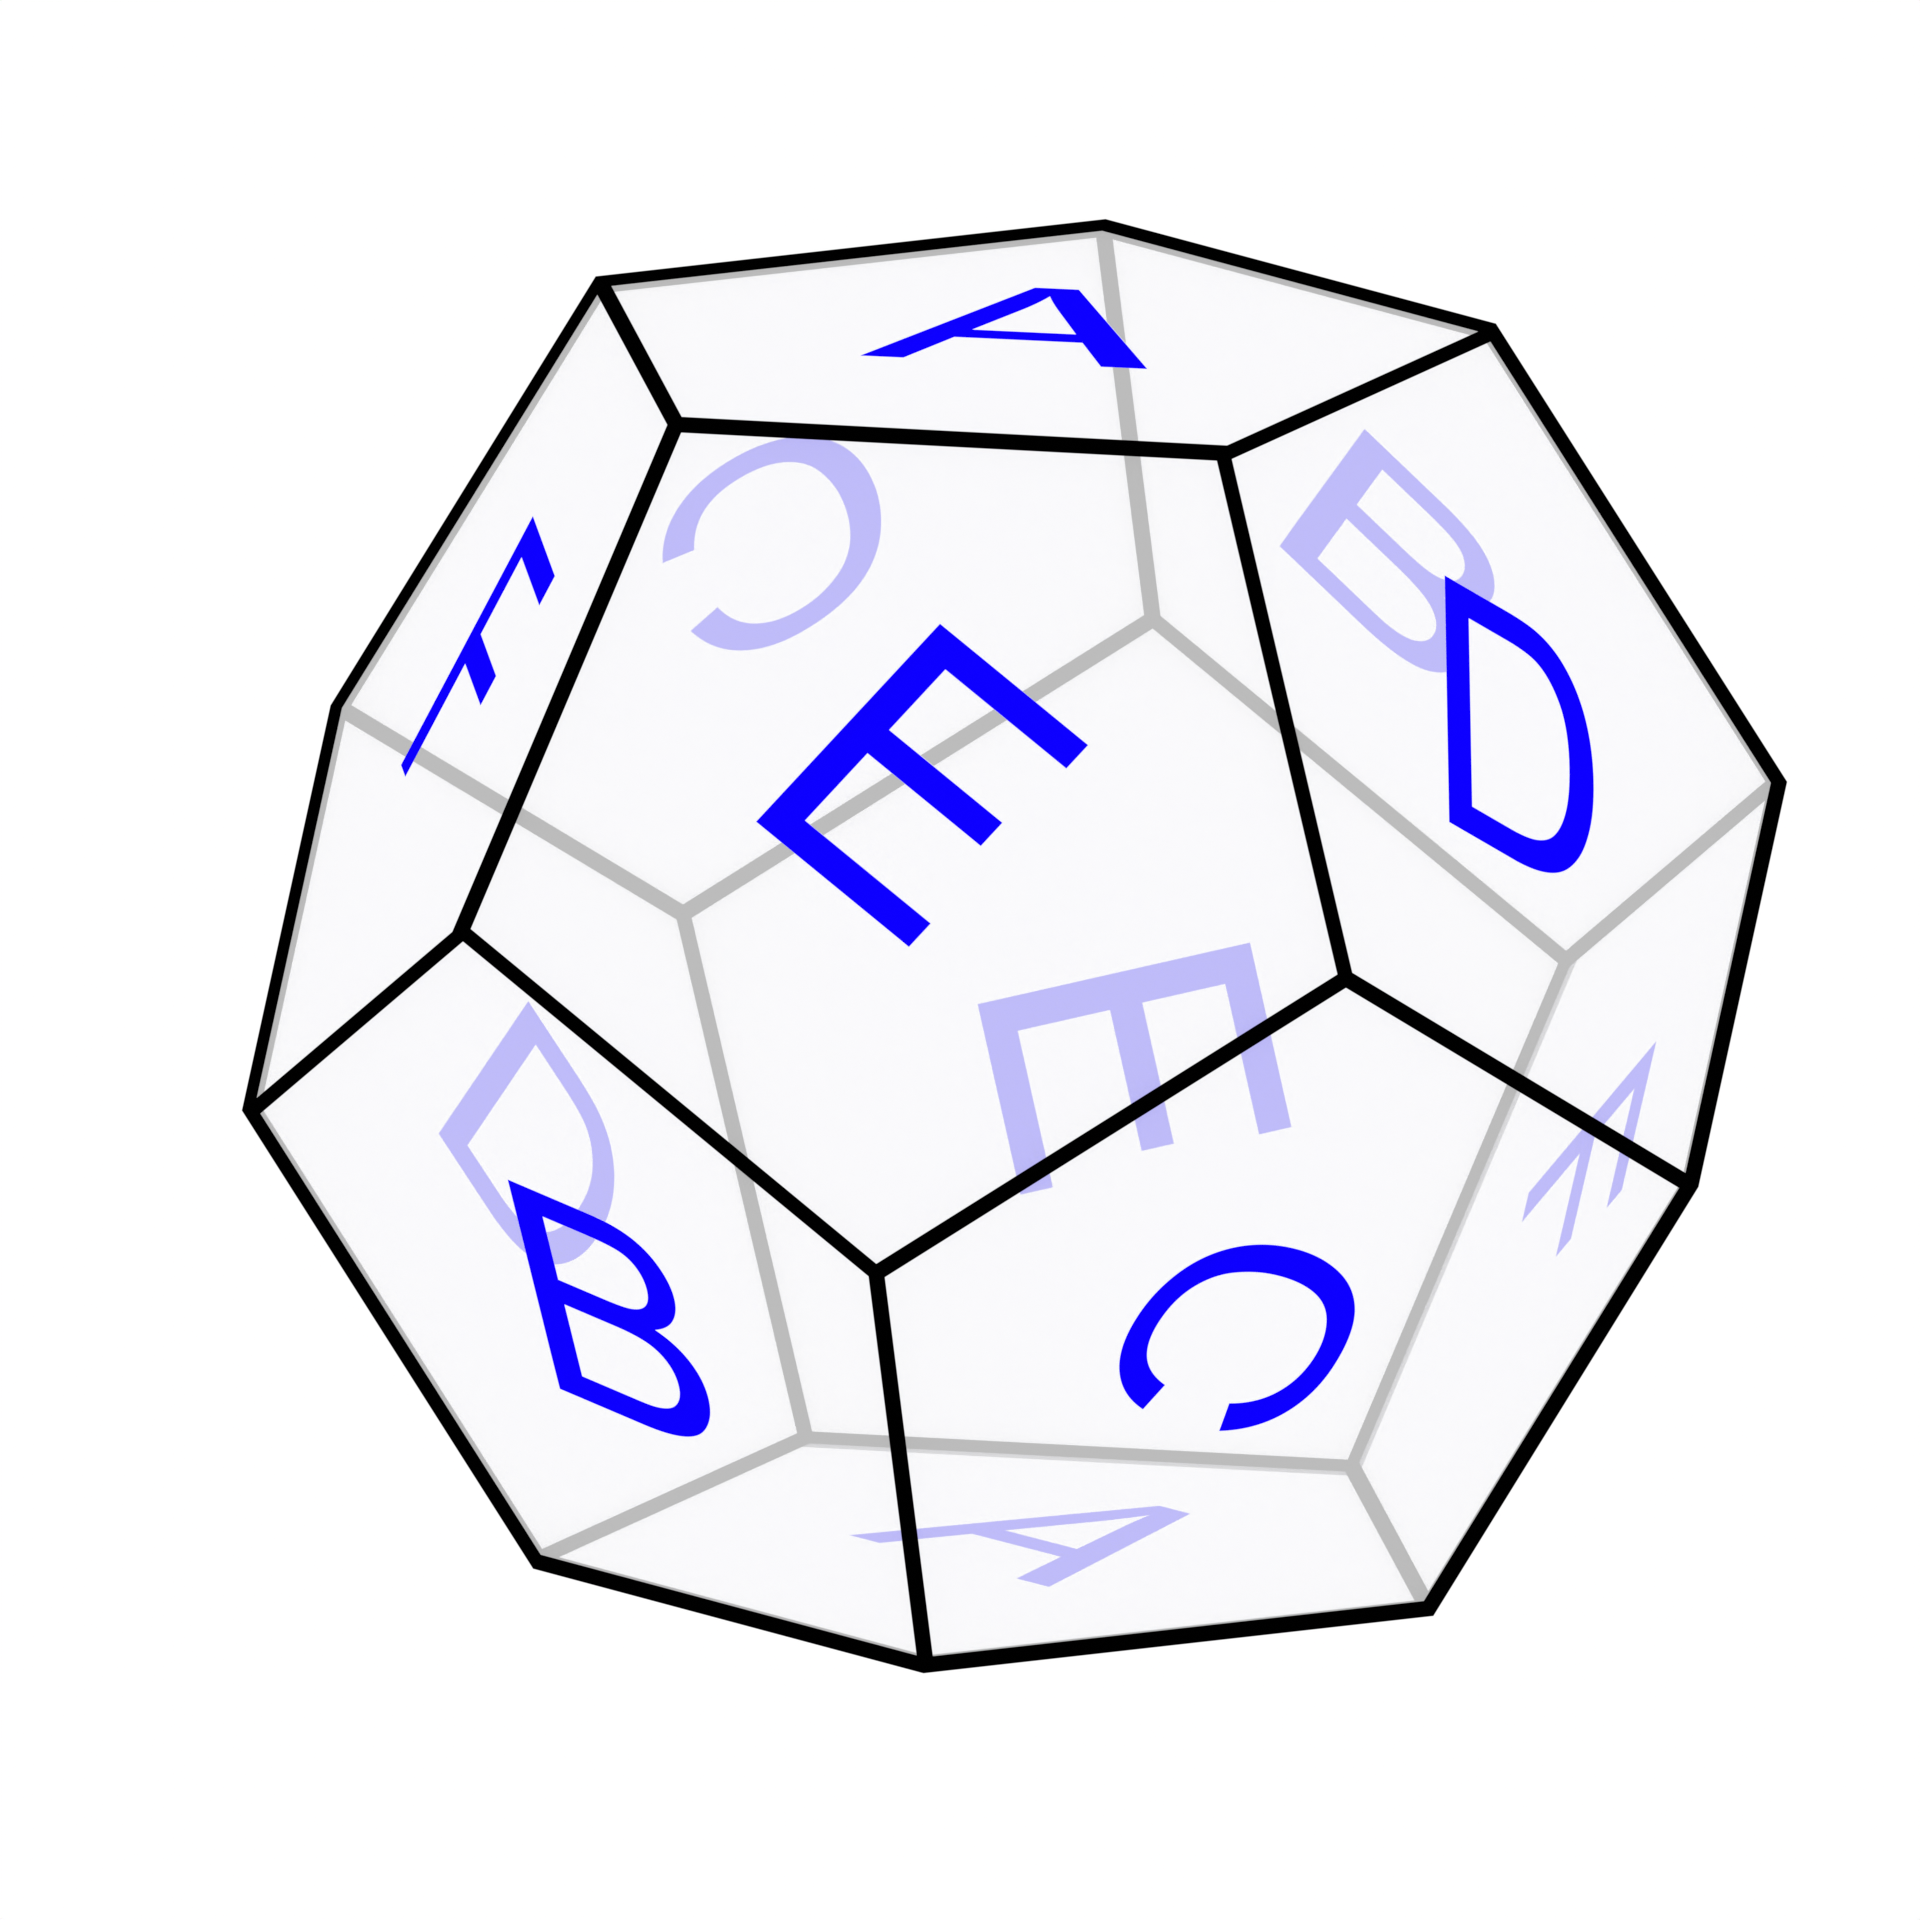
\includegraphics[width=2in]{graphics/temp-diagrams/dodecahedral-space-geometric-construction.png}
	\caption{Construction of Dodecahedral Space}\label{fig:dodecahedral_space_construction}
\end{figure}

Given this geometric construction, it should be fairly straightforward -- albeit tedious -- to compute the homology of dodecahedral space by means of a cellular decomposition. After such a computation, we would find that:
\begin{proposition}
	Dodecahedral space is a homology $3$-sphere.
\end{proposition}

While the first homology of dodecahedral space is trivial and incapable of differentiating dodecahedral space from a 3-sphere, the fundamental group reveals a much richer geometric structure. If we let $\SO_3$ act on $\R^3$ in the usual way, we can form the symmetry group $\Sym(\mathcal{D})\subset \SO_3$ of orientation preserving orthogonal transformations which leave the dodecahedron $\mathcal{D}$ unchanged. This is known as the \defn{icosahedral group}\footnote{The icosahedron and dodecahedron are dual, so the choice of icosahedral in the name is purely a historical convention.} $\mathrm{I}\subset \SO_3$, a group containing $60$ elements and isomorphic to the alternating group $A_5$. There is a double cover of $\SO_3$ by the $\Spin_3$ Lie group:
\[
	\SU_2\cong \Spin_3\lkxto[2:1] \SO_3
\]
The \defn{binary icosahedral group}, denoted $2\mathrm{I}$, is the preimage of $\mathrm{I}$ under this double cover and hence contains $120$ elements. Since there is an exceptional isomorphism $\SU_2\cong \Spin_3$, the binary icosahedral group admits a representation by unitary complex $2\times 2$ matrices.
We then have:
\begin{proposition}
	The fundamental group of dodecahedral space is the binary icosahedral group.
\end{proposition}
This hints at another interesting fact about the binary icosahedral group -- it is a \defn{perfect group}, which means that it's commutator subgroup is the entire group. By the Hurewicz isomorphism, it would follow that
\[
	\H_1(\mathscr{D}) \cong \Ab\left[ \pi_1(\mathscr{D})\right] \cong 2\mathrm{I}/[2\mathrm{I}, 2\mathrm{I}] = 0
\]
where $\Ab$ denotes the abelianization. This perfectness of the fundamental group thus ``hides'' the non-trivial topology of $\mathscr{D}$ from being detectable by homology. It's interesting to note that dodecahedral space and $S^3$ are the only homology $3$-spheres up to homeomorphism with finite fundamental groups.

There is also a useful construction of dodecahedral space which will later appear in our later study of Brieskorn manifolds in \todo{cite}. If we identify $\SU_2$ with the $3$-sphere of unit quaternions, we obtain the construction:

\begin{proposition}
	There is a diffeomorphism $\mathscr{D} \cong S^3 / 2\mathrm{I}$ expressing dodecahedral space as the quotient of the $3$-sphere under a proper group action by $2\mathrm{I}$.
\end{proposition}

Finally, let's see how the dodecahedral space and binary icosahedral group arises out of the plumbing construction we've worked with thus far.

\todo{write this section}

\begin{proposition}
	There is a diffeomorphism $\mathscr{D}\cong \partial P^4(\E_8)$.
\end{proposition}

\todo{citations}

\begin{remark}
	In the early 2000's, the Wilkinson Microwave Anisotropy Probe (WMAP) was launched to accurately map out the cosmic microwave background, i.e. leftover heat from the Big Bang. The observed lack of temperature correlations above 60$^\circ$ led astrophysicist Jean-Paul Luminet to propose a cosmological model \cite{luminet2003dodecahedral} where the shape of the universe is a dodecahedral space, explaining the lack of large scale correlations by means of the compact topology of space. In such a finite universe, larger temperature correlations simply wouldn't have enough room to form.
	While this model made some predictions aligning with observed cosmological data
	\cite{roukema2008dodecahedral}, higher resolution data by the later Planck spacecraft later seemed to suggest that the observable large scale topology is trivial, leading to the modern prevalence of the $\Lambda$CDM model as a standard model for cosmology.
\end{remark}

